\subsection{Cardinality and Infinite Sets}

% **Role:** rigorous language of real and complex analysis.
%
% Countable/uncountable sets, Cantor arguments, cardinal comparison, countable operations.


Cardinality begins with the idea that a set is counted by matching it with another set, not by naming its elements. The function language in Definition \ref{def:functions-images-preimages}, the power-set notation in Definition \ref{def:analysis-sets-and-operations}, and the bijection language in Definition \ref{def:injective-surjective-bijective} are the standing prerequisites for this subsection.

\begin{definition} \label{def:cardinality-equivalence} \hlt{Same Cardinality}\\
Two sets $A$ and $B$ have \hlt{same cardinality}, or are \hlt{equivalent}, if $\exists$ a bijection $f:A\to B$. Then $A\sim_{\#}B$.\\
The relation $\sim_{\#}$ is an equivalence relation: $A\sim_{\#}A$ by identity map, symmetry follows from Theorem \ref{thm:bijective-iff-invertible-function}, and transitivity follows by composing bijections.
\end{definition}

\begin{definition} \label{def:finite-countable-uncountable}\label{def:cardinality-core-definitions-source-todo} \hlt{Finite, Countable, and Uncountable}\\
Set $J_0\defeq\emptyset$, and for $n\geq1$ set $J_n\defeq\{1,2,\ldots,n\}$. A set $A$ is
\begin{enumerate}[label=(\roman*)]
\setlength{\itemsep}{0pt}
\item \hlt{finite} if $A\sim_{\#} J_n$ for some $n\in\N$;
\item \hlt{infinite} if it is not finite;
\item \hlt{countable} if $A\sim_{\#} \N$;
\item \hlt{uncountable} if it is neither finite nor countable;
\item \hlt{at most countable} if it is finite or countable.
\end{enumerate}
Countable sets are also called enumerable or denumerable.
\end{definition}

\begin{principle} \label{princ:well-ordering-natural-numbers} \hlt{Well-Ordering of $\N$}\\
Every nonempty subset of $\N$ has a least element, justifying first unused indices, first repeated values, and increasing listings of infinite subsets of $\N$.
\end{principle}

\begin{proposition} \label{prop:finite-cardinality-well-defined} \hlt{Finite Cardinality is Well Defined}\\
If $A\sim_{\#}J_m$ and $A\sim_{\#}J_n$, then $m=n$. Thus $\#A=n$ is well defined for finite sets.
\begin{proof}
By transitivity of $\sim_{\#}$, it suffices to prove $J_m\sim_{\#}J_n\Rightarrow m=n$. Induct on $m$.\\
For $m=0$, only $J_0=\emptyset$ is bijective to $J_0$.\\
If $m,n\geq1$ and $f:J_m\to J_n$ is bijective, remove $m$ and its partner $f(m)$. The remaining sets are bijective and relabel as $J_{m-1}$ and $J_{n-1}$, so induction gives $m-1=n-1$, hence $m=n$.\\
\hlt{Structural Commentary}: Finite counting is invariant under bijection.\\
\hlt{Key Insight}: Remove one matched element and count down.
\end{proof}
\end{proposition}

\begin{definition} \label{def:sequence-as-enumeration} \hlt{Sequences as Enumerations}\\
A \hlt{sequence} in set $A$ is $x:\N\to A$, written $(x_n)$, where $x_n\defeq x(n)$. Terms of sequence need not be distinct.\\
If $A$ is countable, then its elements can be arranged as a sequence with distinct terms. Conversely, a sequence whose terms are distinct and whose range is $A$ gives a bijection $\N\to A$.
\end{definition}

\begin{example} \label{ex:integers-are-countable} \hlt{The Integers Are Countable}\\
The set $\Z$ is countable. One explicit enumeration is given by
\begin{align}
f(n)=
\begin{cases}
\frac{n}{2}, & n \text{ even},\\[2mm]
-\frac{n-1}{2}, & n \text{ odd},
\end{cases}
\qquad n\in\N. \nonumber
\end{align}
This lists $\Z$ as $0,1,-1,2,-2,3,-3,\ldots$.
\end{example}

\begin{theorem} \label{thm:infinite-subset-of-countable-is-countable} \hlt{Infinite Subsets of Countable Sets}\\
Every infinite subset of a countable set is countable.
\begin{proof}
Let $E\subseteq A$ be infinite, and enumerate $A$ by distinct terms $(x_n)$. Let $n_1<n_2<\cdots$ be exactly the indices for which $x_{n_k}\in E$, listed in increasing order. Then $k\mapsto x_{n_k}$ is a bijection from $\N$ onto $E$.\\
\hlt{Structural Commentary}: The proof keeps only the entries of the original enumeration that land in $E$.\\
\hlt{Key Insight}: An infinite subset of an enumeration inherits an enumeration by first appearances.
\end{proof}
\end{theorem}

\begin{proposition} \label{prop:subsets-and-images-at-most-countable} \hlt{Subsets and Images of At Most Countable Sets}\\
Let $A$ be at most countable.
\begin{enumerate}[label=(\roman*)]
\setlength{\itemsep}{0pt}
\item If $B\subseteq A$, then $B$ is at most countable.
\item If $f:A\to Y$ is a function, then $f(A)$ is at most countable.
\end{enumerate}
\begin{proof}
If $A$ is finite, both claims are immediate. Otherwise write $A=\{a_n:n\in\N\}$ with the $a_n$ distinct.
\begin{enumerate}[label=(\roman*)]
\setlength{\itemsep}{0pt}
\item If $B$ is infinite, let $I_B\defeq\{n:a_n\in B\}=\{n_1<n_2<\cdots\}$.\\
Then $k\mapsto a_{n_k}$ bijects $\N$ onto $B$; the finite case is trivial.
\item Let $I\defeq\{n:f(a_n)\notin\{f(a_m):m<n\}\}$. By (i), $I$ is at most countable, $n\mapsto f(a_n)$ bijects $I$ onto $f(A)$.
\end{enumerate}
\hlt{Structural Commentary}: Subsets select indices; images select first appearances.\\
\hlt{Key Insight}: Subsets and images preserve at-most-countability.
\end{proof}
\end{proposition}

\begin{theorem} \label{thm:countable-union-of-countable-sets}\label{thm:cardinality-main-results-source-todo} \hlt{Countable Union of Countable Sets}\\
Let $(E_n)$ be a sequence of countable sets and put $S\defeq\bigcup\limits_{n=1}^{\infty}E_n$. Then $S$ is countable.
\begin{proof}
Enumerate each $E_n$ as $(x_{nk})_{k\in\N}$. Reading array $(x_{nk})$ by diagonals gives a sequence whose image is $S$.\\
Thus $S$ is at most countable by Proposition \ref{prop:subsets-and-images-at-most-countable}.\\
Since $E_1\subseteq S$ and $E_1$ is countable, $S$ is infinite; hence $S$ is countable.\\
\hlt{Structural Commentary}: The diagonal order turns a two-indexed list into a one-indexed list.\\
\hlt{Key Insight}: Countably many countable rows can still be scanned by one sequence.
\end{proof}
\end{theorem}

\begin{corollary} \label{cor:at-most-countable-union-at-most-countable} \hlt{At Most Countable Unions}\\
If $A$ is at most countable and $B_\alpha$ is at most countable for each $\alpha\in A$, then $\bigcup\limits_{\alpha\in A}B_\alpha$ is at most countable.
\begin{proof}
Let $T\defeq\bigcup\limits_{\alpha\in A}B_\alpha$. If $T=\emptyset$, we are done. Otherwise enumerate the nonempty sets among the $B_\alpha$ as $B_{\alpha_1},B_{\alpha_2},\ldots$, repeating indices if needed, and list each $B_{\alpha_j}$ as $(b_{jk})_{k\in\N}$.\\
A diagonal scan of $(b_{jk})$ has image $T$, so Proposition \ref{prop:subsets-and-images-at-most-countable} makes $T$ at most countable.\\
\hlt{Structural Commentary}: Finite pieces cause no difficulty; they can be embedded into countable rows.\\
\hlt{Key Insight}: At most countable indexing $+$ at most countable indexed sets gives at most countable total set.
\end{proof}
\end{corollary}

\begin{theorem} \label{thm:finite-tuples-over-countable-set-countable} \hlt{Finite Tuples over a Countable Set}\\
Let $A$ be countable. For each fixed $n\in\N$, the set of all $n$-tuples $(a_1,\ldots,a_n)$ with $a_k\in A$ is countable.
\begin{proof} Let $B_n\defeq \{(a_1,\ldots,a_n): a_k\in A\}$, $B_1=A$. If $B_{n-1}$ is countable, $B_n=\bigcup\limits_{b\in B_{n-1}}\{(b,a):a\in A\}$, each set $\{(b,a):a\in A\}$ is equivalent to $A$. Hence $B_n$ is countable by Theorem \ref{thm:countable-union-of-countable-sets}.\\
\hlt{Structural Commentary}: Build an $n$-tuple by appending one coordinate to an $(n-1)$-tuple.\\
\hlt{Key Insight}: Induction plus countable unions controls finite products.
\end{proof}
\end{theorem}

\begin{corollary} \label{cor:countable-cartesian-products} \hlt{Countable Cartesian Products}\\
If $A,B$ are at most countable, then $A\times B$ is at most countable.\\
If $A,B$ are countable and nonempty, then $A\times B$ is countable. Hence $\N\times\N$ is countable.
\begin{proof}
For $a\in A$, $\{a\}\times B\sim B$, and $A\times B=\bigcup\limits_{a\in A}\bigl(\{a\}\times B\bigr)$, thus $A\times B$ at most countable (Corollary \ref{cor:at-most-countable-union-at-most-countable}). If $A,B$ are countable and $b_0\in B$, then $a\mapsto(a,b_0)$ injects $A$ into $A\times B$, so $A\times B$ is infinite; hence it is countable.\\
\hlt{Structural Commentary}: A product is a countable union of countable slices.\\
\hlt{Key Insight}: Two countable coordinates can still be scanned by one sequence.
\end{proof}
\end{corollary}

\begin{corollary} \label{cor:rationals-countable} \hlt{The Rationals Are Countable}\\
The set $\Q$ is countable.
\begin{proof}
Let $D\defeq\{(a,b)\in\Z\times\Z:a\neq0\}$ and $\pi:D\to\Q$ by $\pi(a,b)=b/a$.\\
Since $\Z$ is countable, Corollary \ref{cor:countable-cartesian-products} and Proposition \ref{prop:subsets-and-images-at-most-countable} make $D$ at most countable. Since $\pi(D)=\Q$, Proposition \ref{prop:subsets-and-images-at-most-countable} makes $\Q$ at most countable. As $\Z\subseteq\Q$, it is countable.\\
\hlt{Structural Commentary}: Repeated fractions only add repetitions to the list.\\
\hlt{Key Insight}: Countable pairs produce countably many rational values.
\end{proof}
\end{corollary}

\begin{theorem} \label{thm:cantor-power-set-theorem} \hlt{Cantor's Theorem}\\
For every set $X$, no function $f:X\to\mathcal{P}(X)$ is surjective. Hence $X$ and $\mathcal{P}(X)$ cannot have the same cardinality.
\begin{proof}
Suppose $f:X\to\mathcal{P}(X)$ were surjective, and set $D\defeq\{x\in X:x\notin f(x)\}$.\\
Since $D\subseteq X$, we have $D\in\mathcal{P}(X)$, so surjectivity gives $D=f(a)$ for some $a\in X$.\\
But then $a\in D \Longleftrightarrow a\notin f(a) \Longleftrightarrow a\notin D$, a contradiction.\\
\hlt{Structural Commentary}: The diagonal set is defined to disagree with each proposed row at its own index.\\
\hlt{Key Insight}: Power sets are too large to be exhausted by their base set.
\end{proof}
\end{theorem}

\begin{figure}[H]
  \centering
  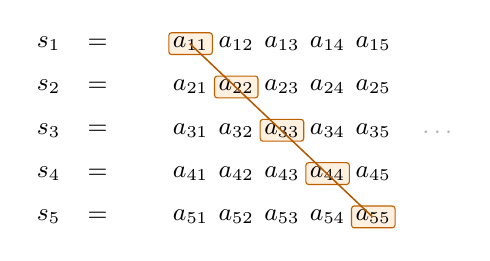
\begin{tikzpicture}[
  every node/.style={font=\small},
  digit/.style={font=\small},
  diagonal/.style={draw=orange!75!black, fill=orange!12, rounded corners=1pt, inner sep=1.5pt},
  guide/.style={orange!70!black, line width=0.55pt}
]
  \foreach \row/\name in {1/s_1,2/s_2,3/s_3,4/s_4,5/s_5} {
    \node[anchor=east] at (0,-0.55*\row) {$\name$};
    \node at (0.35,-0.55*\row) {$=$};
  }

  \foreach \row in {1,...,5} {
    \foreach \col in {1,...,5} {
      \node[digit] at (0.95+0.58*\col,-0.55*\row) {$a_{\row\col}$};
    }
  }

  \foreach \row in {1,...,5} {
    \node[diagonal] at (0.95+0.58*\row,-0.55*\row) {$a_{\row\row}$};
  }
  \draw[guide] (1.52,-0.55) -- (3.84,-2.75);

  \node[anchor=west, gray!60] at (4.35,-1.68) {$\cdots$};
\end{tikzpicture}

  \caption{Cantor diagonalization: $s(n)=1-a_{nn}$ differs from row $s_n$ at position $n$.}
  \label{fig:cantor-diagonal-binary-sequences}
\end{figure}

\begin{theorem} \label{thm:binary-sequences-uncountable} \hlt{Binary Sequences Are Uncountable}\\
Let $A$ be the set of all sequences whose terms are the digits $0$ and $1$. Then $A$ is uncountable.
\begin{proof}
Suppose $A$ were countable, $A=\{s_1,s_2,\ldots\}$ with $s_n=(s_n(k))_{k\in\N}$. Define $s\in A$ by $s(k)\defeq 1-s_k(k)$.\\
Then $s(n)\neq s_n(n)$ for every $n$, so $s\neq s_n$ for all $n$. Hence $s\notin A$, a contradiction. Thus $A$ is uncountable.\\
\hlt{Structural Commentary}: The construction attacks the diagonal of a proposed enumeration.\\
\hlt{Key Insight}: A sequence can be built to escape every row of a countable list.
\end{proof}
\end{theorem}

\begin{figure}[H]
  \centering
  \begin{tikzpicture}[
  >=Stealth,
  every node/.style={font=\small},
  layer/.style={draw=gray!45, fill=gray!8, rounded corners=2pt, minimum width=0.86cm, minimum height=0.42cm},
  farrow/.style={->, blue!60!black, line width=0.55pt},
  garrow/.style={->, orange!75!black, line width=0.55pt},
  restarrow/.style={<->, gray!65, line width=0.55pt}
]
  \foreach \i/\name in {0/A_0,1/A_1,2/A_2,3/A_3} {
    \node[layer] (A\i) at (1.25*\i,1.0) {$\name$};
  }
  \node at (4.45,1.0) {$\cdots$};
  \node[layer] (As) at (5.6,1.0) {$A_*$};

  \foreach \i/\name in {0/B_0,1/B_1,2/B_2,3/B_3} {
    \node[layer] (B\i) at (1.25*\i,0) {$\name$};
  }
  \node at (4.45,0) {$\cdots$};
  \node[layer] (Bs) at (5.6,0) {$B_*$};

  \draw[farrow] (A0) -- node[left] {$f$} (B0);
  \draw[garrow] (B0) -- node[above left=-1pt] {$g$} (A1);
  \draw[farrow] (A1) -- node[left] {$f$} (B1);
  \draw[garrow] (B1) -- node[above left=-1pt] {$g$} (A2);
  \draw[farrow] (A2) -- node[left] {$f$} (B2);
  \draw[garrow] (B2) -- node[above left=-1pt] {$g$} (A3);
  \draw[farrow] (A3) -- node[left] {$f$} (B3);
  \draw[restarrow] (As) -- node[right] {$g^{-1}$} (Bs);

  \node[blue!55!black] at (1.85,-0.55) {$h=f$ on the layers};
  \node[gray!55] at (5.6,-0.55) {$h=g^{-1}$};
\end{tikzpicture}

  \caption{Schroeder--Bernstein: alternating images leave a remainder paired by $g^{-1}$.}
  \label{fig:schroeder-bernstein-ladder}
\end{figure}


\begin{theorem} \label{thm:schroeder-bernstein} \hlt{Schroeder--Bernstein Theorem}\\
If there are injections $f:A\to B$ and $g:B\to A$, then there is a bijection $h:A\to B$.
\begin{proof}
Let $A_0\defeq A\setminus g(B)$, and recursively define $B_n\defeq f(A_n)$ and $A_{n+1}\defeq g(B_n)$.\\
The sets $A_n$ are pairwise disjoint: if $A_i\cap A_j\neq\emptyset$ with $i<j$, then $i=0$ already contradicts $A_j\subseteq g(B)$; if $i>0$, injectivity of $g$ and then $f$ steps backward to $A_{i-1}\cap A_{j-1}\neq\emptyset$, and iteration gives the same contradiction.\\
Since $f$ is injective, the sets $B_n=f(A_n)$ are pairwise disjoint as well.\\
Let $A_*\defeq A\setminus\bigcup\limits_{n\geq0}A_n$ and $B_*\defeq B\setminus\bigcup\limits_{n\geq0}B_n$. The map $g$ restricts to a bijection $B_*\to A_*$.\\
Indeed, $g(B_*)$ avoids every $A_n$, while if $a\in A_*$ then $a\notin A_0$, so $a=g(b)$ for a unique $b\in B$; this $b$ cannot lie in any $B_n$, otherwise $a\in A_{n+1}$.\\
Define $h(x)\defeq
\begin{cases}
f(x), & x\in\bigcup_{n\geq0}A_n,\\
g^{-1}(x), & x\in A_*,
\end{cases}$, where $g^{-1}$ denotes the inverse of $g:B_*\to A_*$.\\
This maps each $A_n$ bijectively onto $B_n$ and maps $A_*$ bijectively onto $B_*$. Hence $h$ is a bijection $A\to B$.\\
\hlt{Structural Commentary}: Two injections carve both sets into matched layers plus a common remainder.\\
\hlt{Key Insight}: Use $f$ on the escaping layers and $g^{-1}$ on the stable remainder.
\end{proof}
\end{theorem}

\begin{principle} \label{princ:axiom-of-choice-analysis} \hlt{Choice Principle}\\
For nonempty sets $\{X_i\}_{i\in I}$, the axiom of choice asserts $\exists c:I\to\bigcup\limits_{i\in I}X_i$ such that $c(i)\in X_i\ \forall i\in I$.\\
Use direct construction for finite or explicit choices; use choice only for arbitrary simultaneous choices.
\end{principle}

\begin{definition} \label{def:ordered-set-vocabulary} \hlt{Ordered Set Vocabulary}
\begin{enumerate}[label=(\roman*)]
\setlength{\itemsep}{0pt}
\item $\leq_X$ is a \hlt{partial order} if it is reflexive, anti-symmetric, and transitive.
\item $C\subseteq X$ is a \hlt{chain} if any two points of $C$ are comparable.
\item $X$ is \hlt{well-ordered} if every nonempty $Y\subseteq X$ has a least element.
\item For $Y\subseteq X$, $u\in X$ is an \hlt{upper bound} if $y\leq_Xu$ for all $y\in Y$.
\item $m\in Y$ is \hlt{maximal} if no $y\in Y$ satisfies $m<_Xy$; minimal is dual.
\end{enumerate}
\end{definition}

\begin{principle} \label{princ:zorns-lemma} \hlt{Zorn's Lemma}\\
If a nonempty partially ordered set $X$ has the property that every chain in $X$ has an upper bound in $X$, then $X$ contains a maximal element. This is equivalent in strength to the axiom of choice, Principle \ref{princ:axiom-of-choice-analysis}.
\end{principle}

\begin{method} \label{meth:cardinality-proof-patterns}\label{meth:cardinality-proof-patterns-source-todo} \hlt{Cardinality Proof Patterns}
\begin{enumerate}[label=(\roman*)]
\setlength{\itemsep}{0pt}
\item Same cardinality: construct a bijection.
\item Countable: construct a sequence whose range contains every element.
\item Uncountable: show every proposed sequence misses some element.
\item Choice/maximality: cite Principle \ref{princ:axiom-of-choice-analysis} for arbitrary simultaneous choices and Principle \ref{princ:zorns-lemma} for maximal elements in partially ordered sets.
\end{enumerate}
\hlt{Key Idea}: Use maps: bijections prove equal cardinality, enumerations $\N\to A$ prove countability, and diagonal arguments show every proposed enumeration misses an element.
\end{method}
